\section{Polar Codes}

\subsection{Channel Polarization - The Idea}

Polar Codes are a family of linear codes that are the first family of codes to reach the Shannon Limit aka 'channel capacity'. They were created by Arikan in 2008 and later mathematically proven to reach the limit in 2013. \\

%This paper intuitively explains the basis of Polar codes and the properties in information theory that allow their functionality, not the implementation. \\

Arikan initially had the goal of finding a way to compress a message $u$ that is $n$ bits long. He paired up each bit in the input message as ($U$, $V$). He tried encoding the bits by simply performing the XOR operation between the two bits,  $(U, V) \to U \oplus V$, however, one bit of information was lost as a result. Therefore, he added another value that is linear and different from $U \oplus V$, simply choosing a copy of the second bit. So far, Arikan has encoded, $(U, V) \to (U \oplus V, V)$. Given the pair $U \oplus V$ and $V$, the operation is easily reversible, and therefore no information is lost. \\

One crucial property Arikan noticed is that, although he didn't succeed in compressing the information, he encoded it in a way that altered the entropy of each bit-channel (meaning each bit now has it's own probability and channel capacity). But how do the entropies of each new bit-channel change? \\

\textbf{Statement 1}: Given $U$ and $V$ are independant Bernoulli random variables with $0 \le p \le \frac{1}{2}$, we want to show that for $ U \oplus V$, the new probability of error $p'$ is greater than $p$. \\


Given that $U$ and $V$ are mutually exclusive independant events, we can compute $p'$ like so:
\[
 p' = \P(U \oplus V = 1) = \underbrace{\P(U=1, V=0)}_{p(1-p)} + \overbrace{\P(U=0, V=1)}^{(1-p)p}    = 2p(1-p).\\[-0.6cm]
\]


% \begin{align*}
%     p' &= \P(U \oplus V = 1) \\
%     &= \underbrace{\P(U=1, V=0)}_{p(1-p)} + \overbrace{\P(U=0, V=1)}^{(1-p)p}    \\
%     &= 2p(1-p).
% \end{align*}

Then, the difference $p' - p = \overbrace{p}^{\leq \frac 1 2}(1-\underbrace{2p}_{\leq 1})$ is a positive quantity. This asserts the claim. Next,


\textbf{Statement 2}: 
\begin{itemize}
    \item[a)] The first sub-channel's entropy increases: $H(U \oplus V) > H(U)$ and $H(U\oplus V) > H(V)$.
    \item[b)] The second sub-channel's entropy decreases: $H(V \mid U \oplus V) < H(U)$ and $H(V \mid U \oplus V) < H(V)$.
\end{itemize}

From now on we denote $h(p)$ as the entropy of a Bernoulli random variable with parameter $p$.

The first statement is trivial; $p' > p$ implies $h(p') > h(p)$. For the second statement, recall that the joint entropy of two independent random variables is the sum of their entropies:
\[
H(U,V) = H(U) + H(V)
\]

where $H(U, V)$ is the joint entropy of both $U$ and $V.$ After Arıkan’s transformation, we have the new pair $(U \oplus V, V)$. It is reversible to $(U, V),$ and so $H(U \oplus V, V)$ should equal $H(U, V)$. The chain rule of entropy yields
\[
\underbrace{H(U \oplus V, V)}_{=2h(p)} = \overbrace{H(U \oplus V)}^{=h(p')} + H(V \mid U \oplus V)
\]

\footnote{Can you figure out why $H(U \oplus V, V) = 2h(p)$?} As a result, we can see 

\[
H(V|U \oplus V) = 2h(p) - h(p') < h(p)
\]

As a final result, we observe how elements in the first group have entropy $H(U \oplus V)  > h(p)$ and elements of the second sub-channel $H(V|U \oplus V) < h(p)$. So the first sub-channel has a larger entropy, and so its channel capacity decreases, and vice versa for the second channel. This manipulation of channel capacities is called \textit{channel polarization} - see Figure \ref{fig:localpolar}, and it's the key idea behind Polar Codes. 

\newpage
\begin{figure}[H]
    \centering
    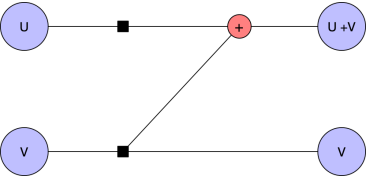
\includegraphics[width=0.5\linewidth]{images/localpolarization.png}
    % \caption{Local Polarization \cite{sudan}}
    \label{fig:localpolar}
\end{figure}

Consider what would happen if we recursively applied this algorithm. How would the channel entropies change? Let us take $2^n$ copies of the BSC, called subchannels, and recursively apply the above. We pair up $U$ and $V$, apply the operation, then separate $U \oplus V$ objects and $V$ objects whilst maintaining their order. Repeat this until only $n$ individual bits remain after separation that have either entropy 1 (useless) or entropy 0 (ideal). Observe Figure \ref{fig:polarization} for a visualization.

\begin{figure}
    \centering
    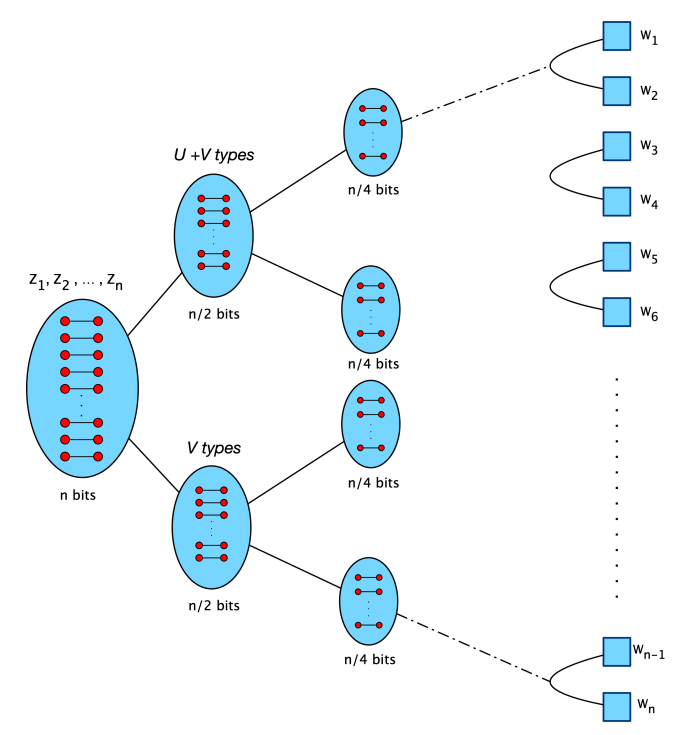
\includegraphics[width=0.5\linewidth]{images/recursiontree.png}
    \caption{Polarization process}
    \label{fig:polarization}
\end{figure}

The final result of this stage is a set of $n$ virtual channels, either with channel capacity 0, 1 or somewhere in between. We select the channels with capacity 1 to send data through and ones with capacity 0 are \textit{frozen}, meaning they are set to 0 and do not store meaningful data.

The careful readers may notice a glaring issue; won't there still be some 'middling' channels that have a mediocre channel capacity of 0.3, 0.6, 0.7, etc. Fortunately, Arikan proved in his paper that as number of bits $N \to \infty$, the fraction of 'middling' virtual channels vanishes, leaving channels with either channel capacity of 0 or 1.

Unfortunately, for a small number of bits, the polarization process results in some virtual channels having a mediocre capacity - 0.3, 0.6, 0.8. 

\subsection{Touching on Implementation and Advantages}

As the operations are all reversible, decoding it is a simple but long algorithm. If we observe Figure \ref{fig:polarization} (the recursive polarization) we can see that $w_{n}$ is exclusively a V-type and does not depend on another bit channel, so it can be used to decode $w_{n-1}$, then $w_{n-1}$ can be used to decode $w_{n-2}$ and so on in a process called successive cancellation decoding which is outside the scope of this paper. \\

The properties of polar codes make them suitable
An advantage of polar codes is that the number of steps to fully polarize the channels is a known value $\log_{2}n$, since the number of copies halves at each stage. \\
